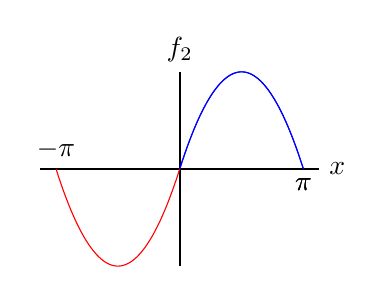
\begin{tikzpicture}[scale=0.5]
% Axis
\draw[thick] (-pi-0.4,0)--(pi+0.4,0) node[right]{$x$};
\draw[thick] (0,-pi*pi/4)--(0,pi*pi/4) node[above]{$f_2$};

\draw[blue, samples=50, domain=0:pi] plot ({\x},{\x * (pi - \x)});

\node[below] at (pi,0) {$\pi$};

\draw[blue, samples=50, domain=0:pi] plot ({\x},{\x * (pi - \x)});
\draw[red, samples=50, domain=-pi:0] plot ({\x},{-(-\x * (pi -( -\x)))});

\node[below] at (pi,0) {$\pi$};
\node[above] at (-pi,0) {$-\pi$};

\end{tikzpicture}
